\section{Model}
The function described in this problem is the following 
\begin{equation*}
\begin{aligned}
    &F(\boldsymbol{x}) = \frac{1}{2}\sum_{k=1}^n f_k^2(\boldsymbol{x}) \\
    &f_k(\boldsymbol{x}) = x_k-1, & k=1 \\
    &f_k(\boldsymbol{x}) = 10(k-1)(x_k-x_{k-1})^2, & 1<k\leq n
\end{aligned}
\end{equation*}
where $n$ is the length of the input vector $\boldsymbol{x}$.
With the given starting point for minimization being 
$$\boldsymbol{x_0}=[-1.2,-1.2,...,-1.2,-1]' \in \mathbbm{R}^n.$$
The gradient of $F(\boldsymbol{x})$ is the following (note that, besides the first and last components, all the others have the same structure).
\begin{equation*}
    \nabla F(\mathbf{x}) = 
    \begin{bmatrix}
        \frac{\partial F}{\partial x_1}(\mathbf{\boldsymbol{x}}) \\
        \vdots \\
        \frac{\partial F}{\partial x_k}(\mathbf{\boldsymbol{x}}) \\
        \vdots \\
        \frac{\partial F}{\partial x_n}(\mathbf{\boldsymbol{x}})
    \end{bmatrix}
    =
    \begin{bmatrix}
        \frac{\partial }{\partial x_1}\frac{1}{2}(f_1^2+f_2^2)(\boldsymbol{x}) \\
        \vdots \\
        \frac{\partial F}{\partial x_k}\frac{1}{2}(f_k^2+f_{k+1}^2)(\boldsymbol{x}) \\
        \vdots \\
        \frac{\partial F}{\partial x_n}\frac{1}{2}f_n^2(\boldsymbol{x})
    \end{bmatrix}
    =
    \begin{bmatrix}
        x_1-1-200\cdot (x_2-x_1)^3 \\
        \vdots \\
        200 \cdot \Big((k-1)^2(x_k-x_{k-1})^3-k^2(x_{k+1}-x_k)^3\Big)\\
        \vdots \\
        200 \cdot (n-1)^2(x_n-x_{n-1})^3
    \end{bmatrix}
\end{equation*}
The Hessian matrix of $F(\boldsymbol{x})$ is sparse since only on three diagonals elements different from zeros are present. They are the following:
\begin{align*}
    \frac{\partial^2 F}{\partial x_1^2} (\boldsymbol{x}) &= 1+600\cdot(x_2-x_1)^2 \\
    \frac{\partial^2 F}{\partial x_k^2} (\boldsymbol{x}) &= 600\cdot\Big((k-1)^2(x_k-x_{k-1})^2+k^2(x_{k+1}-x_k)^2 \Big), \quad 1 < k < n  & \\
    \frac{\partial^2 F}{\partial x_n^2} (\boldsymbol{x}) &=600\cdot(n-1)^2(x_n-x_{n-1})^2 \\
    \frac{\partial^2 F}{\partial x_k \partial x_{k-1}} (\boldsymbol{x}) &= -600\cdot (k-1)^2(x_k-x_{k-1})^2, \quad 1<k\leq n.
\end{align*}
It is easy to notice that $F$, being the sum of squared functions, is always non negative. Furthermore, $F(\boldsymbol{x})=0$ if and only if $\boldsymbol{x}=[1,1,...,1]'$ since $f_1(\boldsymbol{x})^2=0$ if and only if $x_1=1$ and, for every $1<k\leq n$, $f_k(\boldsymbol{x})=0$ if and only if $x_k=x_{k-1}$.

More formally, we can see that $\boldsymbol{x}=[1,1,...,1]'$ solves the equation $\nabla F(\boldsymbol{x})=\boldsymbol{0}$. Since $F$ is convex (being the sum of convex functions) and differentiable, we know that any stationary point is a global minimum point for $F$. 

Then $\boldsymbol{x}=[1,1,...,1]'$ is the only global minimum point for $F$.

We plot the function for $n=2$ in a neighborhood of the minimum point.
\begin{figure}[H]
    \centering
    \begin{subfigure}{0.45\textwidth}
        \centering
        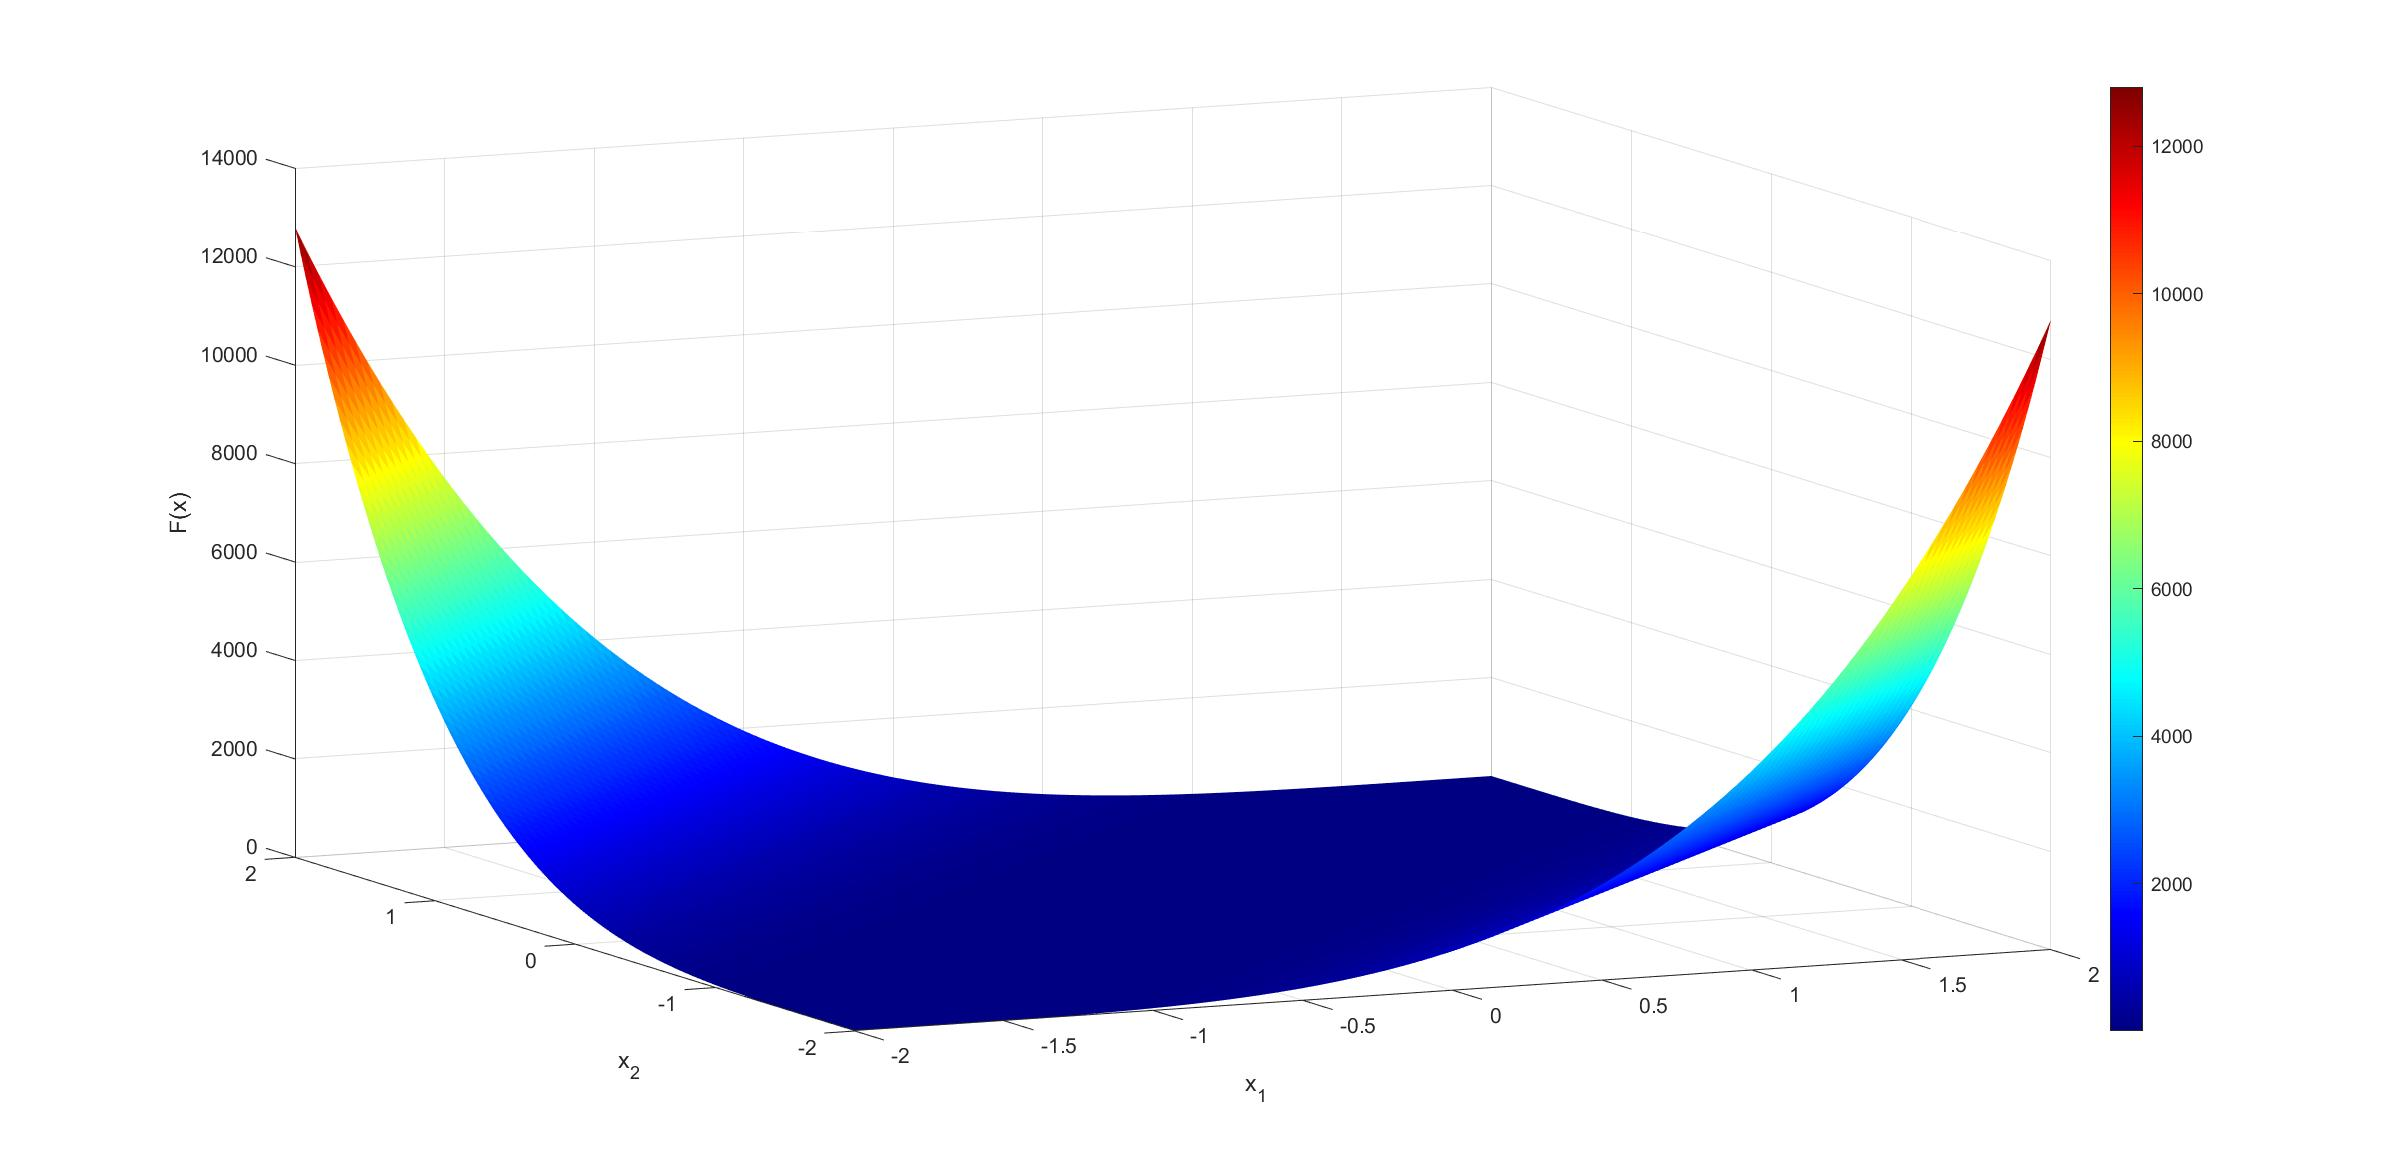
\includegraphics[width=\textwidth]{img/function_pb75_angolo1.jpg}
        \caption{}
    \end{subfigure}
    \begin{subfigure}{0.45\textwidth}
        \centering
        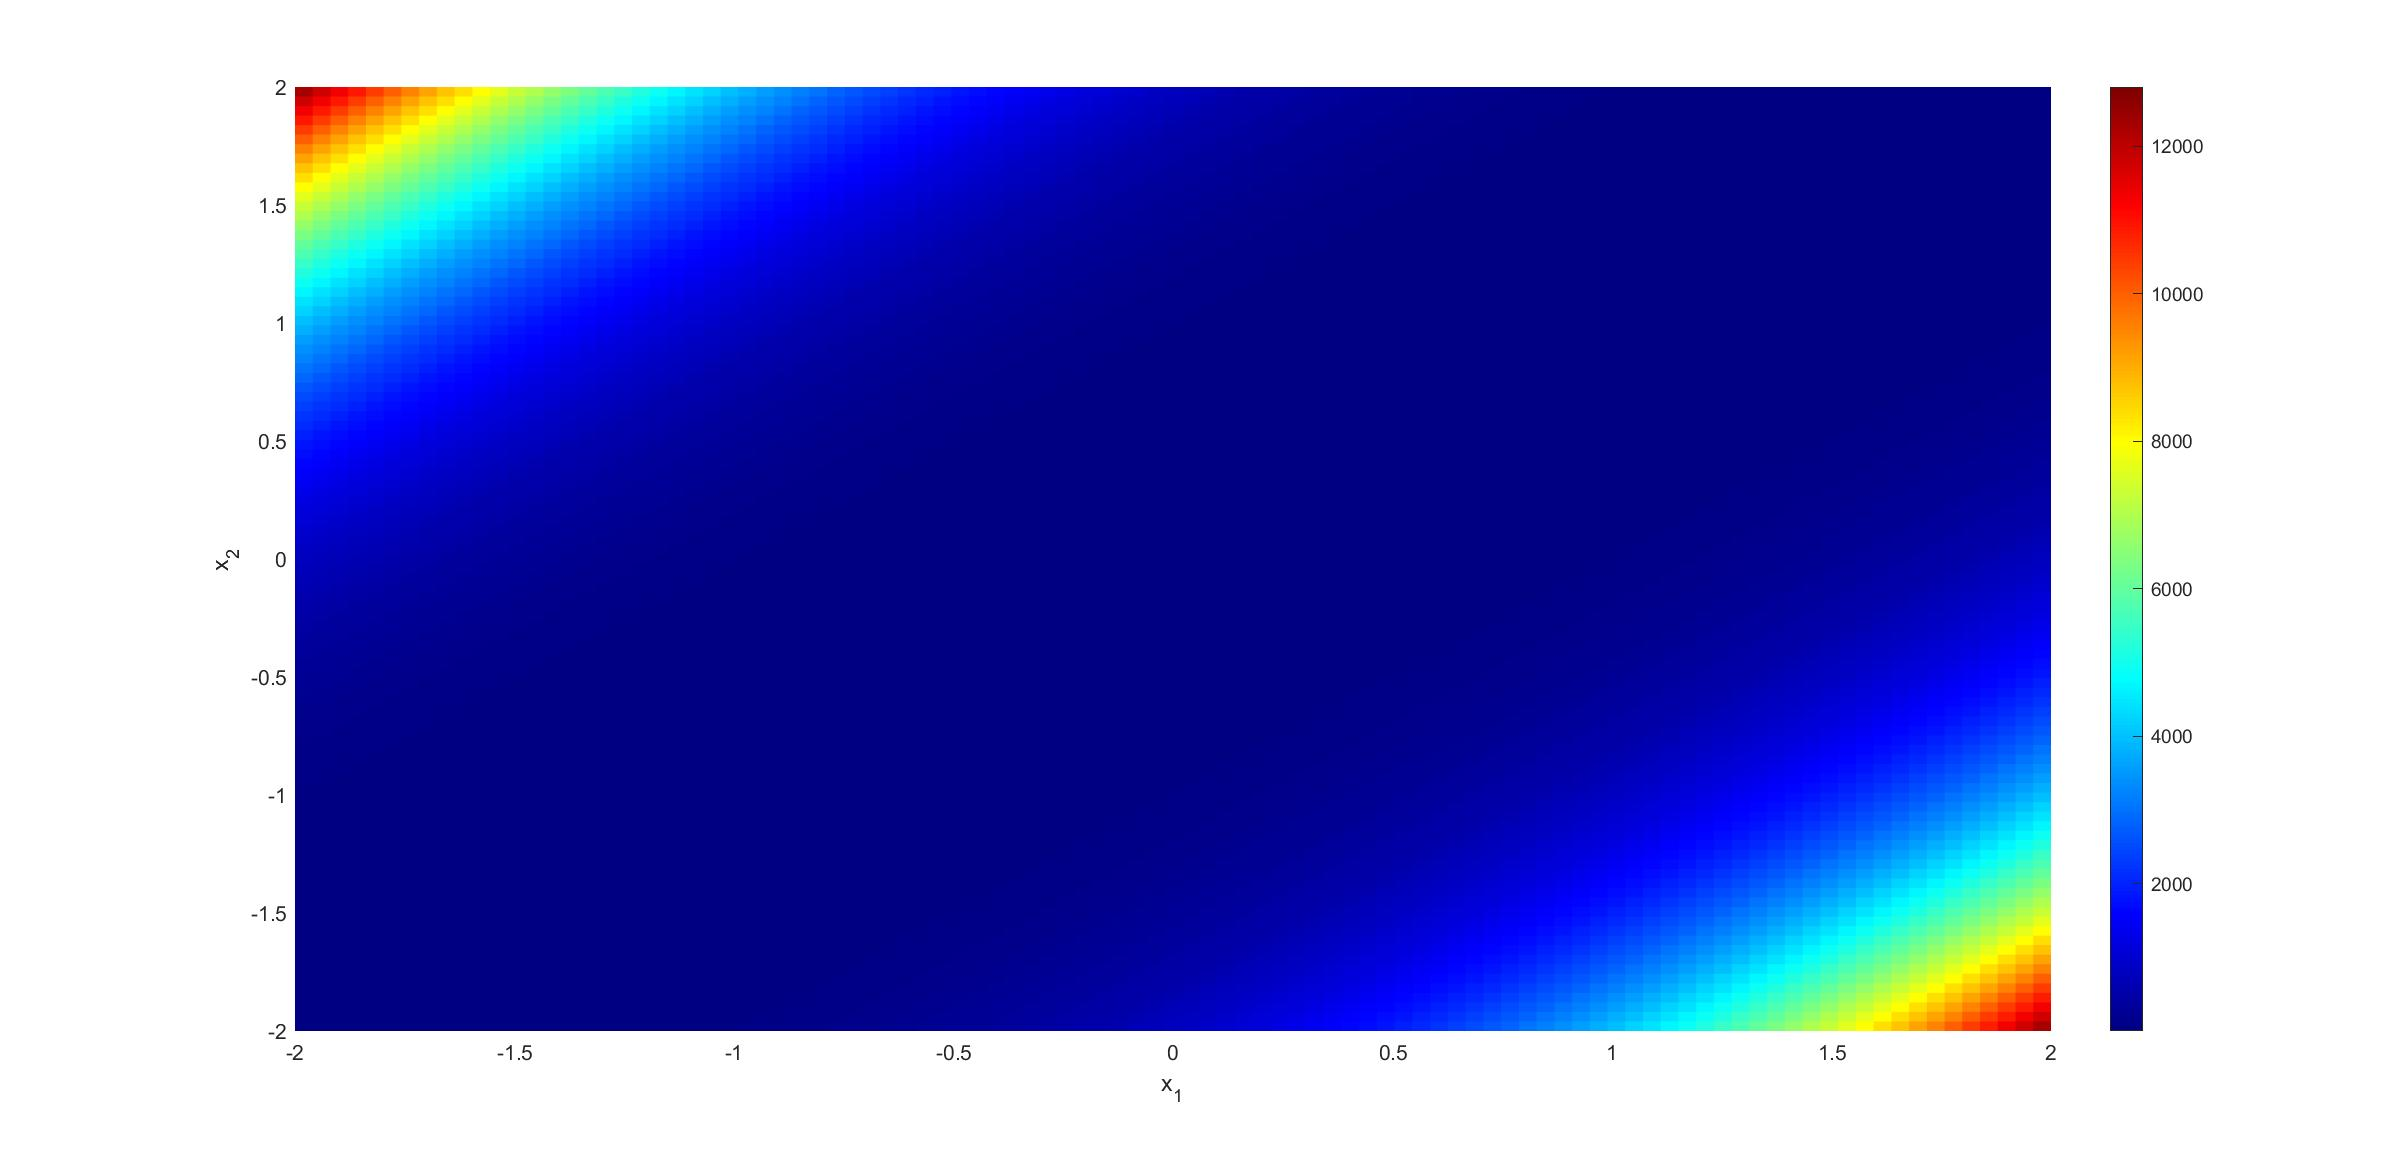
\includegraphics[width=\textwidth]{img/function_pb75_angolo2.jpg}
        \caption{}
    \end{subfigure}
    \caption{function $F(\boldsymbol{x})$ for $n=2$}
\label{fig:funzione 2D pb 75}
\end{figure}
We can easily see that the central area, where the minimum point is located,
is quite flat. This means that the minimization methods used might have some troubles
when reaching this area because they might get stuck before reaching the minimizer.

\section*{Nelder Mead Method}
We runned the minimisation problem with Nelder Mead method using the following parameters:
\begin{eqnarray*}
    \text{reflection } \rho &=& 1.1 \\
    \text{expansion } \chi &=& 2.5 \\
    \text{contraction } \rho &=& 0.6 \\
    \text{shrinking } \rho &=& 0.5.
\end{eqnarray*}
The aim, with this choice, is to try to keep the simplex big enough so that
the method will not get stuck too easily in the almost flat areas of the function's graph.

We now report a table summarizing the results obtained by running the Nelder-Mead method
on the considered problem for dimensions $n=$10, 25, 50 and for a total of 11 starting 
points for each dimension, obtained as perturbations of the given one.

\begin{figure}[H]
    \centering
    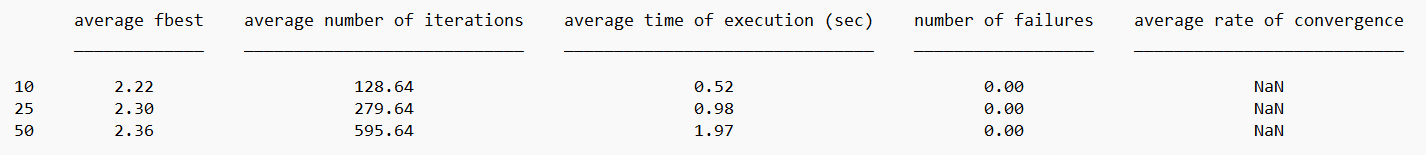
\includegraphics[width=1\textwidth]{img/pb75_table_SX.png}
    \caption{Results obtained by running the Nelder Mead method on problem 75}
\label{pb 75 table SX}
\end{figure}

We notice that the method reports zero failures, which means that it never stopped because of the maximum 
number of iterations allowed (in this case $200\cdot n$) had been reached. However, the best value of the 
function $F$ that has been found is not so close to the expected value (which as observed before should be 0).
The problem is in the starting point. In fact, even with the random perturbations, it always falls in the flat area 
of the function. Tuning the parameters in a way that encourages the expansion of the simplex's area is not enough 
to prevent the method from getting stuck here. It can be seen that, if we use as a staring point for example $[0,0,...,0]'$, 
the results are a bit closer to the exact one (around 0.35). 

The Nelder Mead method does not guarantee convergence and it is sensitive to the starting point and this becomes evident 
in this optimisation problem.
